%%
%% Automatically generated file from DocOnce source
%% (https://github.com/hplgit/doconce/)
%%

% #define PREAMBLE

% #ifdef PREAMBLE
%-------------------- begin preamble ----------------------

\documentclass[%
oneside,                 % oneside: electronic viewing, twoside: printing
final,                   % draft: marks overfull hboxes, figures with paths
10pt]{article}

\listfiles               %  print all files needed to compile this document

\usepackage{relsize,makeidx,color,setspace,amsmath,amsfonts,amssymb}
\usepackage[table]{xcolor}
\usepackage{bm,ltablex,microtype}

\usepackage[pdftex]{graphicx}

\usepackage[T1]{fontenc}
%\usepackage[latin1]{inputenc}
\usepackage{ucs}
\usepackage[utf8x]{inputenc}

\usepackage{lmodern}         % Latin Modern fonts derived from Computer Modern

% Hyperlinks in PDF:
\definecolor{linkcolor}{rgb}{0,0,0.4}
\usepackage{hyperref}
\hypersetup{
    breaklinks=true,
    colorlinks=true,
    linkcolor=linkcolor,
    urlcolor=linkcolor,
    citecolor=black,
    filecolor=black,
    %filecolor=blue,
    pdfmenubar=true,
    pdftoolbar=true,
    bookmarksdepth=3   % Uncomment (and tweak) for PDF bookmarks with more levels than the TOC
    }
%\hyperbaseurl{}   % hyperlinks are relative to this root

\setcounter{tocdepth}{2}  % levels in table of contents

% Tricks for having figures close to where they are defined:
% 1. define less restrictive rules for where to put figures
\setcounter{topnumber}{2}
\setcounter{bottomnumber}{2}
\setcounter{totalnumber}{4}
\renewcommand{\topfraction}{0.95}
\renewcommand{\bottomfraction}{0.95}
\renewcommand{\textfraction}{0}
\renewcommand{\floatpagefraction}{0.75}
% floatpagefraction must always be less than topfraction!
% 2. ensure all figures are flushed before next section
\usepackage[section]{placeins}
% 3. enable begin{figure}[H] (often leads to ugly pagebreaks)
%\usepackage{float}\restylefloat{figure}

% --- fancyhdr package for fancy headers ---
\usepackage{fancyhdr}
\fancyhf{} % sets both header and footer to nothing
\renewcommand{\headrulewidth}{0pt}
\fancyfoot[LE,RO]{\thepage}
% Ensure copyright on titlepage (article style) and chapter pages (book style)
\fancypagestyle{plain}{
  \fancyhf{}
  \fancyfoot[C]{{\footnotesize \copyright\ 2018-2019, Christian Forssén. Released under CC Attribution-NonCommercial 4.0 license}}
%  \renewcommand{\footrulewidth}{0mm}
  \renewcommand{\headrulewidth}{0mm}
}
% Ensure copyright on titlepages with \thispagestyle{empty}
\fancypagestyle{empty}{
  \fancyhf{}
  \fancyfoot[C]{{\footnotesize \copyright\ 2018-2019, Christian Forssén. Released under CC Attribution-NonCommercial 4.0 license}}
  \renewcommand{\footrulewidth}{0mm}
  \renewcommand{\headrulewidth}{0mm}
}

\pagestyle{fancy}


% prevent orhpans and widows
\clubpenalty = 10000
\widowpenalty = 10000

% --- end of standard preamble for documents ---


\usepackage[swedish]{babel}

\raggedbottom
\makeindex
\usepackage[totoc]{idxlayout}   % for index in the toc
\usepackage[nottoc]{tocbibind}  % for references/bibliography in the toc

%-------------------- end preamble ----------------------

\begin{document}

% matching end for #ifdef PREAMBLE
% #endif

\newcommand{\exercisesection}[1]{\subsection*{#1}}

\input{newcommands_keep}

% ------------------- main content ----------------------



% ----------------- title -------------------------

\thispagestyle{empty}

\begin{center}
{\LARGE\bf
\begin{spacing}{1.25}
Learning from data: Assigning probabilities
\end{spacing}
}
\end{center}

% ----------------- author(s) -------------------------

\begin{center}
{\bf Christian Forssén}
\end{center}

    \begin{center}
% List of all institutions:
\centerline{{\small Department of Physics, Chalmers University of Technology, Sweden}}
\end{center}
    
% ----------------- end author(s) -------------------------

% --- begin date ---
\begin{center}
Sep 29, 2019
\end{center}
% --- end date ---

\vspace{1cm}


% !split
\section{Ignorance pdfs: Indifference and translation groups}

\begin{itemize}
\item Consider a six-sided dice

\item How do we assign $p(X_i|I)$, $i \in \{1, 2, 3, 4, 5, 6\}$?

\item We do know $\sum_i p(X_i|I) = 1$

\item Invariance under labeling $\Rightarrow p(X_i|I)=1/6$
\begin{itemize}

  \item provided that the prior information $I$ says nothing that breaks the symmetry.
\end{itemize}

\noindent
\end{itemize}

\noindent
% !split
\subsection{Location invariance}
Indifference to a shift $x_0$ for a location parameter $x$ implies that
\[
p(x|I) dx \approx p(x+ x_0|I) d(x+x_0) =  p(x+ x_0|I) dx,
\]
in the allowed range.

\begin{itemize}
\item Invariance under origin position $\Rightarrow p(x|I) =  p(x+ x_0|I)$, i.e., $p(x|I) = \mathrm{constant}$.
\begin{itemize}

  \item Provided that the prior information $I$ says nothing that breaks the symmetry.

\end{itemize}

\noindent
\item The pdf will be zero outside the allowed range (specified by $I$).
\end{itemize}

\noindent
% !split
\subsection{Scale invariance}

Indifference to a re-scaling $\lambda$ of a scale parameter $x$ implies that
\[
p(x|I) dx \approx p(\lambda x|I) d(\lambda x) =  \lambda p(\lambda x|I) dx,
\]
in the allowed range.

\begin{itemize}
\item Invariance under re-scaling $\Rightarrow p(x|I) \propto 1/x$. 
\begin{itemize}

  \item Provided that the prior information $I$ says nothing that breaks the symmetry.

\end{itemize}

\noindent
\item The pdf will be zero outside the allowed range (specified by $I$).

\item This prior is often called a \emph{Jeffrey's prior}; it represents a complete ignorance of a scale parameter within an allowed range.

\item It is equivalent to a uniform pdf for the logarithm: $p(\log(x)|I) = \mathrm{constant}$
\begin{itemize}

  \item as can be verified with a change of variable $y=\log(x)$, see lecture notes on error propagation.
\end{itemize}

\noindent
\end{itemize}

\noindent
\paragraph{Example: Straight-line model.}
Consider the theoretical model $y_\mathrm{th}(x) = \theta_1  x  + \theta_0$.

\begin{itemize}
\item Would you consider the intercept $\theta_0$ a location or a scale parameter, or something else?

\item Would you consider the slope $\theta_1$ a location or a scale parameter, or something else?
\end{itemize}

\noindent
Consider also the statistical model for the observed data $y_i = y_\mathrm{th}(x_i) + \epsilon_i$, where we assume independent, Gaussian noise $\epsilon_i \sim \mathcal{N}(0, \sigma^2)$.
\begin{itemize}
\item Would you consider the standard deviation $\sigma$ a location or a scale parameter, or something else?
\end{itemize}

\noindent
% !split
\subsection{Symmetry invariance}

\begin{itemize}
\item In fact, by symmetry indifference we could as well have written the linear model as $x_\mathrm{th}(y) = \theta_1'  y  + \theta_0'$

\item We would then equate the probability elements for the two models $p(\theta_0, \theta_1 | I) d\theta_0 d\theta_1 = q(\theta_0', \theta_1' | I) d\theta_0' d\theta_1'$.

\item The transformation gives $(\theta_0', \theta_1') = (-\theta_1^{-1}\theta_0, \theta_1^{-1})$.
\end{itemize}

\noindent
This change of variables implies that
\[
q(\theta_0', \theta_1' | I) = p(\theta_0, \theta_1 | I) \left| \frac{d\theta_0 d\theta_1}{d\theta_0' d\theta_1'} \right|,
\]
where the (absolute value of the) determinant of the Jacobian is
\[
\left| \frac{d\theta_0 d\theta_1}{d\theta_0' d\theta_1'} \right| 
= \mathrm{abs} \left( 
\begin{vmatrix}
\frac{\partial \theta_0}{\partial \theta_0'} & \frac{\partial \theta_0}{\partial \theta_1'} \\
\frac{\partial \theta_1}{\partial \theta_0'} & \frac{\partial \theta_1}{\partial \theta_1'} 
\end{vmatrix}
\right)
= \frac{1}{\left( \theta_1' \right)^3}.
\]

\begin{itemize}
\item In summary we find that $\theta_1^3 p(\theta_0, \theta_1 | I) = p(-\theta_1^{-1}\theta_0, \theta_1^{-1}|I).$

\item This functional equation is satisfied by
\end{itemize}

\noindent
\[
p(\theta_0, \theta_1 | I) \propto \frac{1}{\left( 1 + \theta_1^2 \right)^{3/2}}.
\]

% !split

\begin{figure}[!ht]  % 
  \centerline{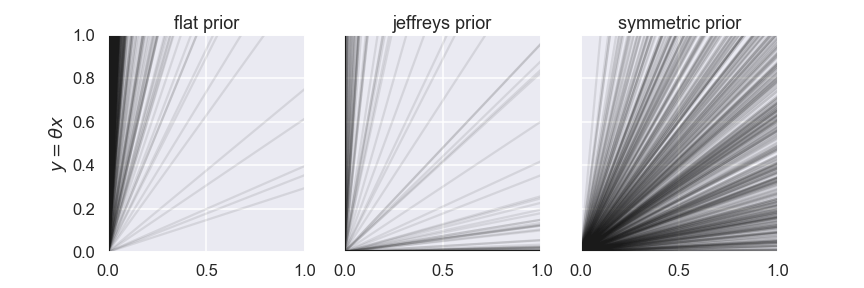
\includegraphics[width=0.8\linewidth]{fig/slope_priors.png}}
  \caption{
  100 samples of straight lines with intercept 0 and slope from three different pdfs.
  }
\end{figure}
%\clearpage % flush figures 



% !split
\section{The principle of maximum entropy}

Having dealt with ignorance, let us move on to a more enlightened situation.

Consider a die with the usual six faces that was rolled a very large number of times. Suppose that we were only told that the average number of dots was 2.5. What (discrete) pdf would we assign? I.e. what are the probabilities $\{ p_i \}$ that the face on top had $i$ dots after a single throw?

% !split
The available information can be summarized as follows
\[
\sum_{i=1}^6 p_i = 1, \qquad \sum_{i=1}^6 i p_i = 2.5
\]
This is obviously not a normal die, with uniform probability $p_i=1/6$, since the average result would then be 3.5. But there are many candidate pdfs that would reproduce the given information. Which one should we prefer?

% !split
It turns out that there are several different arguments that all point in a direction that is very familiar to people with a physics background. Namely that we should prefer the probability distribution that maximizes an entropy measure, while fulfilling the given constraints. 

% !split
\subsection{The entropy of Scandinavians}

Let's consider another pdf assignment problem. This is originally the \emph{kangaroo problem} (Gull and SKilling, 1984), but adapted here to a local context. The problem is stated as follows:

\begin{description}
\item[Information:] 
  70\% of all Scandinavians have blonde hair, and 10\% of all Scandinavians are left handed.

\item[Question:] 
  On the basis of this information alone, what proportion of kangaroos are both blonde and left handed?
\end{description}

\noindent
% !split
We note that for any one given Scandinavian there are four distinct possibilities: 
\begin{enumerate}
\item Blonde and left handed (probability $p_1$).

\item Blonde and right handed (probability $p_2$).

\item Not blonde and left handed (probability $p_3$).

\item Not blonde and right handed (probability $p_4$).
\end{enumerate}

\noindent
% !split
The following 2x2 contingency table



\begin{tabular}{lcc}
\hline
\multicolumn{1}{c}{  } & \multicolumn{1}{c}{ Left handed } & \multicolumn{1}{c}{ Right handed } \\
\hline
Blonde     & $p_1$       & $p_2$        \\
Not blonde & $p_3$       & $p_4$        \\
\hline
\end{tabular}


\noindent
% !split
can be written in terms of a single variable $x$ due to the normalization condition $\sum_{i=1}^4 p_i = 1$, and the available information $p_1 + p_2 = 0.7$ and $p_1 + p_3 = 0.1$



\begin{tabular}{lcc}
\hline
\multicolumn{1}{c}{  } & \multicolumn{1}{c}{ Left handed } & \multicolumn{1}{c}{ Right handed } \\
\hline
Blonde     & $0 \le x \le 0.1$ & $0.7-x$      \\
Not blonde & $0.1-x$           & $0.2+x$      \\
\hline
\end{tabular}


\noindent
But which choice of $x$ is preferred?

% !split
\subsection{The monkey argument}

A model for assigning probabilities to $M$ different alternatives that satisfy some constraint as described by $I$: 
\begin{itemize}
\item Monkeys throwing $N$ balls into $M$ equally sized boxes.

\item The normalization condition $N = \sum_{i=1}^M n_i$.

\item The fraction of balls in each box gives a possible assignment for the corresponding probability $p_i = n_i / M$.

\item The distribution of balls $\{ n_i \}$ is therefore a candidate pdf $\{ p_i \}$.

\item The resulting pdf might not be consistent with the constraints of $I$, however, in which case it should be rejected as a possible candidate.

\item After many such trials, some distributions will be found to come up more often than others. The one that appears most frequently (and satisfies $I$) would be a sensible choice for $p(\{p_i\}|I)$.
\end{itemize}

\noindent
% !split
\begin{itemize}
\item The number of micro-states, $W$, as a function of $\{p_i\}$ is
\end{itemize}

\noindent
\[
\log(W(\{n_i\})) = \log(N!) − \sum_{i=1}^M \log(n_i!) 
\approx N\log(N) - \sum_{i=1}^M n_i\log(n_i),
\]
  where we have used the Stirling approximation $\log(n!) \approx n\log(n) - n$ for large numbers, and a cancellation of two terms. 

% !split
\begin{itemize}
\item There are $M^N$ different ways to distribute the balls.

\item The micro-states $\{ n_i\}$ are connected to the pdf $\{ p_i \}$, so the frequency of a given pdf is given by
\end{itemize}

\noindent
\[
\log(F(\{p_i\})) \approx -N \log(M) + N\log(N) - \sum_{i=1}^M n_i\log(n_i)
\]

Substituting $p_i = n_i/N$, and using the normalization condition finally gives
\[
\log(F(\{p_i\})) \approx -N \log(M) - N \sum_{i=1}^M p_i\log(p_i)
\]

% !split
We note that $N$ and $M$ are constants so that the pdf is given by the $\{ p_i \}$ that maximizes
\[
S = - \sum_{i=1}^M p_i\log(p_i).
\]
You might recognise this quantity as the \emph{entropy} from statistical mechanics. The interpretation of entropy in statistical mechanics is the measure of uncertainty, which remains about a system after its observable macroscopic properties, such as temperature, pressure and volume, have been taken into account. For a given set of macroscopic variables, the entropy measures the degree to which the probability of the system is spread out over different possible microstates. Specifically, entropy is a logarithmic measure of the number of micro-states with significant probability of being occupied $S = -k_B \sum_i p_i \log(p_i)$, where $k_B$ is the Boltzmann constant.

% !split
\paragraph{Why maximize the entropy?}
\begin{itemize}
\item Information theory: maximum entropy=minimum information (Shannon, 1948).

\item Logical consistency (Shore {\&} Johnson, 1960).

\item Uncorrelated assignments related monotonically to $S$ (Skilling, 1988).
\end{itemize}

\noindent
Consider the third argument. Let us check it empirically to the problem of hair colour and handedness of Scandinavians. We are interested in determining $p_1 \equiv p(L,B|I) \equiv x$, the probability that a Scandinavian is both left-handed and blonde. However, in this simple example we can immediately realize that the assignment $p_1=0.07$ is the only one that implies no correlation between left-handedness and hair color. Any joint probability smaller than 0.07 implies that left-handed people are less likely to be blonde, and any larger vale indicates that left-handed people are more likely to be blonde.

% !split
So unless you have specific information about the existence of such a correlation, you should better not build it into the assignment of the probability $p_1$.

\textbf{Question}: Can you show why $p_1 < 0.07$ and $p_1 > 0.07$ corresponds to left-handedness and blondeness being dependent variables?

% !split
Let us now empirically consider a few variational functions of $\{ p_i \}$ and see if any of them gives a maximum that corresponds to the uncorrelated assignment $x=0.07$, which implies $p_1 = 0.07, \, p_2 = 0.63, \, p_3 = 0.03, \, p_4 = 0.27$. A few variational functions and their prediction for $x$ are shown in the following table.



\begin{tabular}{ccc}
\hline
\multicolumn{1}{c}{ Variational function } & \multicolumn{1}{c}{ Optimal x } & \multicolumn{1}{c}{ Implied correlation } \\
\hline
$-\sum_i p_i \log(p_i)$     & 0.070     & None                \\
$\sum_i \log(p_i)$          & 0.053     & Negative            \\
$-\sum_i p_i^2 \log(p_i)$   & 0.100     & Positive            \\
$-\sum_i \sqrt{p_i(1-p_i)}$ & 0.066     & Negative            \\
\hline
\end{tabular}


\noindent

\begin{figure}[!ht]  % 
  \centerline{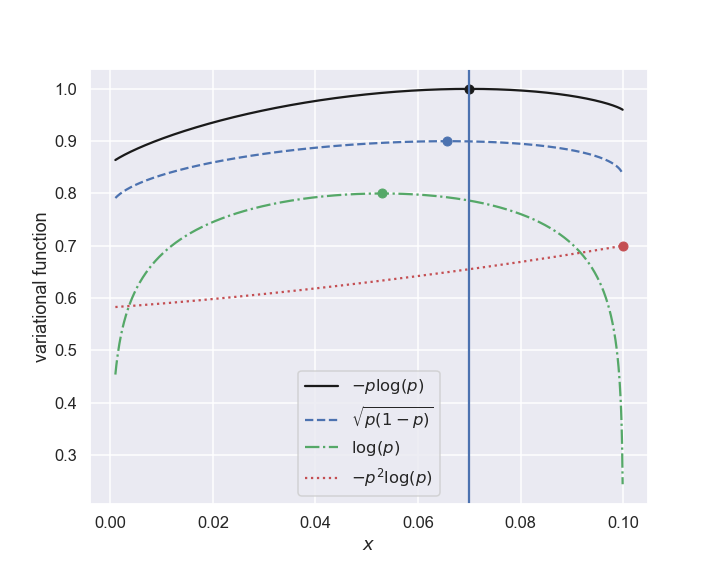
\includegraphics[width=0.8\linewidth]{fig/scandinavian_entropy.png}}
  \caption{
  Four different variational functions $f\left( \{ p_i \} \right)$. The optimal $x$ are shown by circles. The uncorrelated assignment $x=0.07$ is shown by a vertical line.
  }
\end{figure}
%\clearpage % flush figures 


\paragraph{Continuous case.}
Return to monkeys, but now with different probabilities for each bin.Then
\[
S= −\sum_{i=1}^M p_i \log \left( \frac{p_i}{m_i} \right),
\]
which is often known as the \emph{Shannon-Jaynes entropy}, or the \emph{Kullback number}, or the \emph{cross entropy} (with opposite sign).

In the continuous case
\[
S[p]= −\int p(x) \log \left( \frac{p(x)}{m(x)} \right).
\]

\subsection{Derivation of common pdfs using MaxEnt}

\paragraph{Variance and the Gaussian pdf.}
\paragraph{Counting statistics and the Poisson distribution.}

% ------------------- end of main content ---------------

% #ifdef PREAMBLE
\end{document}
% #endif

